\documentclass[9pt,aspectratio=169]{beamer}
\usetheme[progressbar=frametitle,numbering=fraction,block=fill]{metropolis}
% ---------------------------------------------------------------
%  Shared preamble: notation, colours, listings, theorem envs
% ---------------------------------------------------------------
\usepackage[T1]{fontenc}
\usepackage[utf8]{inputenc}
\usepackage{lmodern}
\usepackage{amsmath,amssymb,amsthm}
\usepackage{mathtools}
\usepackage{booktabs}
\usepackage{tabularx}
\usepackage{array}
\usepackage{multirow}
\usepackage{graphicx}
\usepackage{xcolor}
\usepackage{listings}
\usepackage{tikz}
\usetikzlibrary{arrows.meta,positioning,fit,backgrounds,calc,shapes.geometric,decorations.pathreplacing}
\usepackage{caption}

% ---------- palette (colour-blind safe, prints legibly in grey) ----------
\definecolor{cBlue}{HTML}{2B6CB0}
\definecolor{cBlueBg}{HTML}{E7F0FB}
\definecolor{cAmber}{HTML}{B4690E}
\definecolor{cAmberBg}{HTML}{FDF0D5}
\definecolor{cGreen}{HTML}{2F855A}
\definecolor{cGreenBg}{HTML}{E8F5EC}
\definecolor{cPurple}{HTML}{7B3FA0}
\definecolor{cPurpleBg}{HTML}{F6ECFA}
\definecolor{cGrey}{HTML}{6B6B76}
\definecolor{cGreyBg}{HTML}{F1F1F4}
\definecolor{cRed}{HTML}{B03030}
\definecolor{cInk}{HTML}{1A1A1E}

% ---------- U-semiring / Q-expression notation ----------
\newcommand{\Usemi}{\ensuremath{\mathcal{U}}}
\newcommand{\Nbar}{\ensuremath{\overline{\mathbb{N}}}}
\newcommand{\sq}[1]{\ensuremath{\left\lVert #1 \right\rVert}}       % squash
\newcommand{\notu}[1]{\ensuremath{\mathrm{not}(#1)}}                % negation
\newcommand{\ind}[1]{\ensuremath{[\,#1\,]}}                          % indicator
\newcommand{\usum}[1]{\ensuremath{\sum_{#1}}}                        % unbounded sum
\newcommand{\den}[1]{\ensuremath{[\![ #1 ]\!]}}                      % denotation
\newcommand{\Tup}[1]{\ensuremath{\mathrm{Tuple}(#1)}}
\newcommand{\Sumagg}{\ensuremath{\mathrm{Sum}}}
\newcommand{\lam}[2]{\ensuremath{\lambda #1.\,#2}}
\newcommand{\qop}{\ensuremath{\mathrm{QOp}}}
\newcommand{\hop}{\ensuremath{\mathrm{HOp}}}
\newcommand{\zzero}{\ensuremath{\mathbf{0}}}
\newcommand{\oone}{\ensuremath{\mathbf{1}}}

% ---------- inline tags ----------
\newcommand{\udp}{\textsc{UDP}}
\newcommand{\QED}{\textsc{Qed}}
\newcommand{\sqlsolver}{\textsc{SQLSolver}}
\newcommand{\spes}{\textsc{SPES}}
\newcommand{\wetune}{\textsc{WeTune}}
\newcommand{\lia}{\textsf{LIA}}
\newcommand{\liastar}{\textsf{LIA}\ensuremath{^*}}

% ---------- code listings ----------
\lstdefinestyle{sql}{
  language=SQL,
  basicstyle=\ttfamily\small\color{cInk},
  keywordstyle=\color{cBlue}\bfseries,
  commentstyle=\color{cGrey}\itshape,
  stringstyle=\color{cGreen},
  showstringspaces=false,
  breaklines=true,
  columns=fullflexible,
  keepspaces=true,
  morekeywords={ALL,DISTINCT,GROUP,BY,ORDER,INTERSECT,EXCEPT,VALUES,OVER,PARTITION}
}
\lstdefinestyle{plan}{
  basicstyle=\ttfamily\footnotesize\color{cInk},
  breaklines=false,
  columns=fullflexible,
  keepspaces=true,
  escapeinside={(@}{@)}
}
\lstdefinestyle{pseudo}{
  basicstyle=\ttfamily\small\color{cInk},
  keywordstyle=\color{cPurple}\bfseries,
  morekeywords={procedure,function,for,all,if,then,else,return,while,do,end,foreach,and,or,not},
  breaklines=true,
  columns=fullflexible,
  keepspaces=true,
  mathescape=true
}
\lstset{style=sql}

% ---------- boxed "key idea" ----------
\newcommand{\keybox}[2]{%
  \begin{center}
  \begin{tikzpicture}
    \node[draw=cAmber,fill=cAmberBg,line width=0.9pt,rounded corners=3pt,
          inner sep=8pt,text width=0.92\linewidth,align=left]
      {\textbf{\color{cAmber}#1}\\[2pt]#2};
  \end{tikzpicture}
  \end{center}}

\newcommand{\warnbox}[2]{%
  \begin{center}
  \begin{tikzpicture}
    \node[draw=cRed,fill=cGreyBg,line width=0.9pt,rounded corners=3pt,
          inner sep=8pt,text width=0.92\linewidth,align=left]
      {\textbf{\color{cRed}#1}\\[2pt]#2};
  \end{tikzpicture}
  \end{center}}

\usepackage{pgfplots}
\pgfplotsset{compat=1.18}
\usepackage{appendixnumberbeamer}

\setbeamercolor{palette primary}{bg=cInk,fg=white}
\setbeamercolor{frametitle}{bg=cInk,fg=white}
\setbeamercolor{alerted text}{fg=cRed}
\setbeamercolor{block title}{bg=cAmberBg,fg=cAmber}
\setbeamercolor{block body}{bg=cAmberBg!40}
\setbeamertemplate{itemize item}{\color{cBlue}$\blacktriangleright$}
\setbeamertemplate{itemize subitem}{\color{cGrey}--}

\lstset{style=sql,basicstyle=\ttfamily\scriptsize}
\setbeamersize{text margin left=6mm,text margin right=6mm}

% reveal a table row: \onslide must wrap each CELL, never the row's \\
\newcommand{\rowiii}[4]{\onslide<#1->{#2} & \onslide<#1->{#3} & \onslide<#1->{#4}\\}
\newcommand{\rowiv}[5]{\onslide<#1->{#2} & \onslide<#1->{#3} & \onslide<#1->{#4} & \onslide<#1->{#5}\\}

\newcommand{\sectiontitle}[2]{%
  \begin{frame}[standout]
  #1\\[4pt]{\normalsize\normalfont\color{cGreyBg}#2}
  \end{frame}}

\title{Proving SQL Queries Equivalent}
\subtitle{U-expressions, Q-expressions and \liastar{}}
\date{}
\author{}

\begin{document}

\maketitle

% ------------------------------------------------------------------
\begin{frame}[fragile]{The question}
\begin{center}\large
Do these two queries return \alert{the same answer on every database}?
\end{center}
\vspace{2mm}
\begin{columns}[T]
\begin{column}{0.48\textwidth}
\begin{lstlisting}
select x, sum(y)
from R join S on R.x = S.a
group by x
\end{lstlisting}
\end{column}
\begin{column}{0.48\textwidth}
\begin{lstlisting}
select t.x, t.r from
 (select x, sum(y) as r
  from R group by x) t
 join S on t.x = S.a
\end{lstlisting}
\end{column}
\end{columns}
\vspace{4mm}
\onslide<2->{%
\begin{alertblock}{Why anyone cares}
Every engine rewrites your query before running it. A wrong rewrite rule returns wrong
answers, silently, for years.
\end{alertblock}}
\onslide<3->{\centering\small Undecidable in general $\Rightarrow$ every prover here answers
only \textbf{EQUIVALENT} or \textbf{UNKNOWN}.}
\end{frame}

% ------------------------------------------------------------------
\begin{frame}[fragile]{Three systems, one pipeline}
\begin{center}
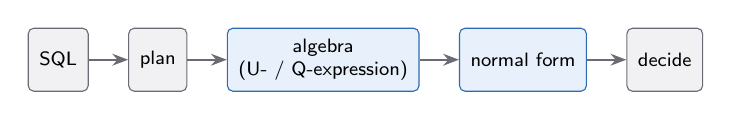
\begin{tikzpicture}[node distance=5mm,font=\scriptsize\sffamily,
  box/.style={draw=cGrey,fill=cGreyBg,rounded corners=2pt,inner sep=4pt,minimum height=8mm,align=center},
  hi/.style ={draw=cBlue,fill=cBlueBg,rounded corners=2pt,inner sep=4pt,minimum height=8mm,align=center},
  ar/.style ={-{Stealth[length=2mm]},cGrey,thick}]
\node[box] (a) {SQL};
\node[box,right=of a] (b) {plan};
\node[hi,right=of b] (c) {algebra\\(U- / Q-expression)};
\node[hi,right=of c] (d) {normal form};
\node[box,right=of d] (e) {decide};
\draw[ar](a)--(b);\draw[ar](b)--(c);\draw[ar](c)--(d);\draw[ar](d)--(e);
\end{tikzpicture}
\end{center}
\vspace{2mm}
\begin{center}\small
\begin{tabular}{@{}llll@{}}
\toprule
 & \textbf{algebra} & \textbf{decision step} & \textbf{innovation}\\
\midrule
\rowiv{2}{\udp{} '18}{U-expression}{syntactic match}{the foundation}
\rowiv{3}{\QED{} '24}{Q-expression}{SMT everywhere}{better \alert{modelling}}
\rowiv{4}{\sqlsolver{} '24}{U-expression}{\liastar{}$\to$\lia{}$\to$SMT}{better \alert{arithmetic}}
\bottomrule
\end{tabular}
\end{center}
\onslide<5->{\vspace{2mm}\centering\small They differ in exactly two places. Everything else follows.}
\end{frame}

\sectiontitle{Part 0}{Bags, counting functions, and $\Sigma$}

% ------------------------------------------------------------------
\begin{frame}[fragile]{A table is a counting function}
\begin{columns}[T]
\begin{column}{0.4\textwidth}
\centering
\begin{tabular}{@{}c|c@{}}
\multicolumn{2}{@{}l}{$R$}\\\toprule
$x$&$y$\\\midrule 1&10\\1&20\\2&30\\\bottomrule
\end{tabular}
\end{column}
\begin{column}{0.58\textwidth}
\onslide<2->{%
\[R(t)=\text{``how many copies of row $t$ are in $R$?''}\]
\vspace{-4mm}
\begin{center}\small
\begin{tabular}{@{}cc@{}}
\toprule $t$ & $R(t)$\\\midrule
$(1,10)$&1\\ $(1,20)$&1\\ $(2,30)$&1\\
$(1,99)$&\alert{0}\\ everything else&\alert{0}\\\bottomrule
\end{tabular}
\end{center}}
\end{column}
\end{columns}
\vspace{3mm}
\onslide<3->{%
\begin{block}{The whole idea}
A query is a \textbf{formula that computes the count of one output row}.\\
Two queries are equivalent iff their formulas agree for every row, on every input.
\end{block}}
\end{frame}

% ------------------------------------------------------------------
\begin{frame}[fragile]{SQL becomes arithmetic}
\begin{center}\small
\begin{tabular}{@{}lll@{}}
\toprule
\textbf{SQL} & \textbf{on counts} & \textbf{why}\\\midrule
\texttt{FROM R}        & $R(t)$ & definition\\
\rowiii{2}{\texttt{WHERE b}}{$\ind{b}\times R(t)$}{multiply by $0$ = delete the row}
\rowiii{3}{\texttt{R, S}}{$R(t_1)\times S(t_2)$}{every pair}
\rowiii{4}{\texttt{UNION ALL}}{$R(t)+S(t)$}{copies accumulate}
\rowiii{5}{\texttt{SELECT x}}{$\usum{y}R(x,y)$}{\alert{forget $y$ $\Rightarrow$ merge counts}}
\rowiii{6}{\texttt{DISTINCT}}{$\sq{R(t)}$}{clamp to $0$ or $1$}
\rowiii{7}{\texttt{NOT EXISTS Q}}{$\notu{\usum{t}Q(t)}$}{$1$ iff the count is $0$}
\bottomrule
\end{tabular}
\end{center}
\onslide<8->{\vspace{3mm}
\begin{alertblock}{No new machinery}
Filtering is multiplication. Joining is multiplication. Union is addition.
That is the entire trick.
\end{alertblock}}
\end{frame}

% ------------------------------------------------------------------
\begin{frame}[fragile]{$\Sigma$ --- ``try every value and add up''}
\[\usum{y}R(1,y)\]
\begin{columns}[T]
\begin{column}{0.44\textwidth}
\onslide<2->{\centering\small
\begin{tabular}{@{}cc@{}}
\toprule $y$ & $R(1,y)$\\\midrule
$\vdots$&$\vdots$\\ 9&0\\ \textbf{10}&\alert{\textbf{1}}\\ 11&0\\ $\cdots$&0\\
\textbf{20}&\alert{\textbf{1}}\\ 21&0\\ $\vdots$&$\vdots$\\\bottomrule
\end{tabular}}
\end{column}
\begin{column}{0.54\textwidth}
\onslide<3->{\textbf{``Isn't that infinite?''}\\[2pt]
No --- a table has finitely many rows, so \alert{almost every term is $0$}.\\[6pt]}
\onslide<4->{Measured in PostgreSQL:\\[2pt]
{\footnotesize
range $0..30$ \quad$\to$\quad \textbf{2}\\
range $-1000..1000$ \quad$\to$\quad \textbf{2}}\\[6pt]}
\onslide<5->{\begin{block}{$\Sigma$ = projection}
Dropping $y$ \textbf{merges} rows that differed only in $y$, so their counts \textbf{add}.
$\usum{y}R(x,y)$ is \texttt{GROUP BY x} $+$ \texttt{COUNT(*)}.
\end{block}}
\end{column}
\end{columns}
\end{frame}

% ------------------------------------------------------------------
\begin{frame}[fragile]{Two things called ``sum''}
\begin{center}\large
\begin{tabular}{@{}lccc@{}}
\toprule
 & \textbf{adds up} & \textbf{SQL} & \textbf{on $\{10,20\}$}\\\midrule
$\usum{y}f(y)$ & multiplicities & \texttt{COUNT(*)} & $1+1=\mathbf{2}$\\[4pt]
\rowiv{2}{$\Sumagg(\lam{y}{f(y)})$}{values $\times$ mult.}{\texttt{SUM(y)}}{$10{\cdot}1+20{\cdot}1=\mathbf{30}$}
\bottomrule
\end{tabular}
\end{center}
\vspace{4mm}
\onslide<3->{%
\begin{alertblock}{$\Sigma$ is COUNT. $\Sumagg$ is SUM.}
And $\lam{y}{R(1,y)}$ \emph{is} a bag --- the bag $\{10,20\}$, written as its counting
function. Aggregates eat whole bags, so their argument must be a function.
\end{alertblock}}
\onslide<4->{\centering\small Double every multiplicity: $\{10,10,20,20\}\Rightarrow\Sumagg=\mathbf{60}$.
\alert{Remember $30\to60$.}}
\end{frame}

\sectiontitle{The running example}{one rewrite, used throughout}

% ------------------------------------------------------------------
\begin{frame}[fragile]{Aggregate pushdown: Calcite's \texttt{AggregateJoinTransposeRule}}
\begin{columns}[T]
\begin{column}{0.5\textwidth}
\textbf{$Q_1$ --- aggregate ABOVE the join}
\begin{lstlisting}
select x, sum(y) as r
from R join S on R.x = S.a
group by x
\end{lstlisting}
\onslide<2->
\begin{lstlisting}[style=plan,basicstyle=\ttfamily\tiny]
LogicalAggregate(group=[{0}],SUMY=[SUM($1)])
  LogicalProject(X=[$0], Y=[$1])
    LogicalJoin(condition=[=($0,$2)])
      TableScan([[R]])
      TableScan([[S]])
\end{lstlisting}
\end{column}
\begin{column}{0.5\textwidth}
\textbf{$Q_2$ --- aggregate BELOW the join}
\begin{lstlisting}
select t.x, t.r from
 (select x, sum(y) as r
  from R group by x) t
 join S on t.x = S.a
\end{lstlisting}
\onslide<2->
\begin{lstlisting}[style=plan,basicstyle=\ttfamily\tiny]
LogicalProject(X=[$0], SUMY=[$1])
  LogicalJoin(condition=[=($0,$2)])
    LogicalAggregate(group=[{0}],SUMY=[SUM($1)])
      TableScan([[R]])
    TableScan([[S]])
\end{lstlisting}
\end{column}
\end{columns}
\onslide<3->{\vspace{2mm}\centering
\alert{\texttt{Aggregate} and \texttt{Join} swap places. That is the entire rewrite.}}
\end{frame}

% ------------------------------------------------------------------
\begin{frame}[fragile]{Calcite fires the rule itself --- and tells us the secret}
\begin{columns}[T]
\begin{column}{0.48\textwidth}
\centering\textbf{\small\texttt{S.A} declared unique}
\begin{lstlisting}[style=plan,basicstyle=\ttfamily\tiny]
LogicalProject(X=[$0], SUMY=[$1])
  LogicalJoin(cond=[=($0,$2)])
    LogicalAggregate(SUMY=[SUM($1)])
      TableScan([[R]])
    LogicalProject(A=[$0])
      TableScan([[S]])
\end{lstlisting}
{\footnotesize\itshape exactly $Q_2$}
\end{column}
\begin{column}{0.5\textwidth}
\onslide<2->
\centering\textbf{\small\texttt{S.A} \emph{not} unique}
\begin{lstlisting}[style=plan,basicstyle=\ttfamily\tiny]
LogicalProject(X=[$0],
   $f4=[CAST(*($1, $3))])
  LogicalJoin(cond=[=($0,$2)])
    LogicalAggregate(SUMY=[SUM($1)])
      TableScan([[R]])
    LogicalAggregate(agg#0=[COUNT()])
      TableScan([[S]])
\end{lstlisting}
{\footnotesize\itshape the aggregate is \alert{multiplied by COUNT}}
\end{column}
\end{columns}
\vspace{2mm}
\onslide<3->{%
\begin{alertblock}{A production optimiser just derived our algebra}
That compensating $\times\,\mathrm{count}$ is literally the $\times\,S(a)$ factor of the
U-expression. The primary key is exactly what lets a prover delete it.
\end{alertblock}}
\end{frame}

% ------------------------------------------------------------------
\begin{frame}[fragile]{One counterexample kills it}
\begin{columns}[T]
\begin{column}{0.34\textwidth}
\centering
$S$ \emph{without} a key\\[2pt]
\begin{tabular}{@{}c|c@{}}\toprule $a$&$b$\\\midrule 1&100\\ \alert{1}&\alert{100}\\\bottomrule\end{tabular}
\end{column}
\begin{column}{0.62\textwidth}
\onslide<2->{\centering
\begin{tabular}{@{}lll@{}}
\toprule & result & rows\\\midrule
$Q_1$ & $(1,\alert{60})$ & 1\\
$Q_2$ & $(1,30),(1,30)$ & \alert{2}\\\bottomrule
\end{tabular}}
\end{column}
\end{columns}
\vspace{4mm}
\onslide<3->{\textbf{Wrong in two independent ways:}}
\begin{itemize}
\item<4-> $Q_1$ joins first $\Rightarrow$ the bag entering \texttt{SUM} becomes
      $\{10,10,20,20\}$ $\Rightarrow$ \alert{the value} is corrupted ($30\to60$).
\item<5-> $Q_2$ aggregates first $\Rightarrow$ \texttt{SUM} sees a clean bag; duplication hits
      \alert{the row count} instead.
\end{itemize}
\onslide<6->{\vspace{2mm}
\begin{alertblock}{The specification}
$Q_1\equiv Q_2$ \textbf{iff} the join column on the right is distinct. A prover that cannot
turn ``primary key'' into algebra cannot prove this; one that proves it without the key is
\emph{unsound}.
\end{alertblock}}
\end{frame}

\sectiontitle{Part I}{U-expressions --- \udp{}, VLDB 2018}

% ------------------------------------------------------------------
\begin{frame}[fragile]{The U-semiring: $(\Usemi,0,1,+,\times,\sq{\cdot},\notu{\cdot},\usum{})$}
$(\Usemi,0,1,+,\times)$ is an ordinary commutative semiring --- arithmetic without
subtraction. Three operators are added.
\vspace{2mm}
\begin{columns}[T]
\begin{column}{0.5\textwidth}
\textbf{squash} $\sq{\cdot}$ \;--\; models \texttt{DISTINCT}
\begin{align*}
\sq{0}&=0 & \sq{1+x}&=1\\
\sq{\sq{x}+y}&=\sq{x+y} & \sq{x}\sq{x}&=\sq{x}\\
\sq{x}\sq{y}&=\sq{xy} & x\sq{x}&=x\\
\multicolumn{4}{l}{$x^2=x\;\Rightarrow\;\sq{x}=x$}
\end{align*}
\end{column}
\begin{column}{0.48\textwidth}
\onslide<2->{\textbf{negation} $\notu{\cdot}$ \;--\; models \texttt{NOT EXISTS}
\begin{align*}
\notu{0}&=1 & \notu{x{+}y}&=\notu{x}\notu{y}\\
\notu{xy}&=\sq{\notu{x}{+}\notu{y}} & \notu{\sq{x}}&=\notu{x}
\end{align*}}
\end{column}
\end{columns}
\vspace{2mm}
\onslide<3->{%
\begin{alertblock}{Why so few, and why all equations?}
Fewer axioms $=$ smaller trusted base $=$ simpler proof search. And every axiom is an
\textbf{identity} $E_1=E_2$, so it can be used as a rewrite rule and checked in Coq.
An order relation $\le$ was deliberately \alert{excluded}.
\end{alertblock}}
\end{frame}

% ------------------------------------------------------------------
\begin{frame}[fragile]{\dots and unbounded summation}
\begin{columns}[T]
\begin{column}{0.48\textwidth}
\textbf{summation} $\usum{}$ \;--\; models projection
\begin{align*}
\usum{t}(f_1{+}f_2)&=\usum{t}f_1+\usum{t}f_2\\
\usum{t_1}\usum{t_2}f&=\usum{t_2}\usum{t_1}f\\
x\usum{t}f&=\usum{t}xf\\
\sq{\usum{t}f}&=\sq{\usum{t}\sq{f}}
\end{align*}
\end{column}
\begin{column}{0.48\textwidth}
\onslide<2->{\textbf{equality}
\begin{align*}
\ind{e_1{=}e_2}+\ind{e_1{\neq}e_2}&=1\\
f(e_1)\ind{e_1{=}e_2}&=f(e_2)\ind{e_1{=}e_2}\\
\usum{t}\ind{t{=}e}&=1
\end{align*}}
\end{column}
\end{columns}
\vspace{2mm}
\onslide<3->{%
\begin{alertblock}{The workhorse (derived from the three equality axioms)}
\centering$\displaystyle\usum{t}\ind{t=e}\times f(t)=f(e)$\\[2pt]
\emph{A summation whose variable is pinned collapses to one value.}
\end{alertblock}}
\onslide<4->{\centering\small A join condition \texttt{ON x = a} creates exactly such a pin
--- which is why join conditions make summations disappear.}
\end{frame}

% ------------------------------------------------------------------
\begin{frame}[fragile]{Keys as an \emph{equation}, not an implication}
\begin{center}\large
$\ind{t.k=t'.k}\times R(t)\times R(t') \;=\; \ind{t=t'}\times R(t)$
\end{center}
\vspace{3mm}
\begin{itemize}
\item<2-> Set $t=t'$: \quad $R(t)^2=R(t)$ \quad$\Rightarrow$\quad $R(t)\in\{0,1\}$ ---
      \alert{no duplicate rows}
\item<3-> Take $t\neq t'$ with $t.k=t'.k$: \quad RHS $=0$ \quad$\Rightarrow$\quad
      $R(t)R(t')=0$ --- \alert{no two rows share a key}
\end{itemize}
\vspace{3mm}
\onslide<4->{%
\begin{block}{Why an equation?}
Everything in a U-semiring must be an \textbf{identity} $E_1=E_2$, so it can be used as a
rewrite rule and checked in Coq. The obvious definition
``$\usum{t}R(t)\ind{t.k=e}\le1$'' needs an \emph{order relation} --- extra axioms the
authors refused to add.
\end{block}}
\end{frame}

% ------------------------------------------------------------------
\begin{frame}[fragile]{A complete proof, by axiom-chasing}
\small $R$ has key $k$; $I$ is an index on $R.a$; goal
\texttt{SELECT * FROM R WHERE a>=12} $\equiv$ index lookup.
\[\den{Q_2}(t)=\usum{t_1,t_2,t_3}\ind{t_2{=}t}\ind{t_1.k{=}t_2.k}\ind{t_1.a{\ge}12}
\ind{t_3.k{=}t_1.k}\ind{t_3.a{=}t_1.a}R(t_3)R(t_2)\]
\begin{enumerate}
\item<2-> $t_1$ has schema $(k,a)$, so the two equalities \alert{determine $t_1$}. Workhorse
      lemma deletes $\usum{t_1}$:
      \[\usum{t_2,t_3}\ind{t_2{=}t}\ind{t_3.k{=}t_2.k}\ind{t_3.a{\ge}12}R(t_3)R(t_2)\]
\item<3-> \alert{KEY identity} on $\ind{t_3.k{=}t_2.k}R(t_3)R(t_2)=\ind{t_2{=}t_3}R(t_2)$:
      \[\usum{t_2,t_3}\ind{t_2{=}t}\ind{t_3.a{\ge}12}R(t_2)\ind{t_2{=}t_3}\]
\item<4-> Workhorse on $t_3$, then $t_2$: \quad
      $\den{Q_2}(t)=\ind{t.a\ge12}\times R(t)=\den{Q_1}(t)$ \hfill$\blacksquare$
\end{enumerate}
\onslide<5->{\begin{alertblock}{The strategy}
SPNF $\to$ delete pinned summations $\to$ apply constraint identities $\to$ compare
\textbf{syntactically}.
\end{alertblock}}
\end{frame}

% ------------------------------------------------------------------
\begin{frame}[fragile]{\udp{}'s two ceilings}
\begin{columns}[T]
\begin{column}{0.5\textwidth}
\textbf{1. Syntactic predicates}\\[4pt]
Comparison is congruence closure over \emph{uninterpreted} functions.
\[\ind{a+b=0} \quad\text{vs}\quad \ind{a=-b}\]
\alert{Does not match.} No arithmetic.\\[4pt]
\onslide<2->{\footnotesize$\Rightarrow$ every system after 2018 calls an SMT solver here.}
\end{column}
\begin{column}{0.48\textwidth}
\onslide<3->{\textbf{2. Aggregates compared out of context}\\[4pt]
$\Sumagg(E_1)=\Sumagg(E_2)$ only by congruence, i.e.\ only if $E_1=E_2$:
\[\lam{y}{R(x,y)\sq{S(x)}} \;\overset{?}{=}\; \lam{y}{R(x,y)}\]
\alert{Genuinely false} standalone --- if $x\notin S$ the left is empty.\\[4pt]
\onslide<4->{\footnotesize$\Rightarrow$ \QED{}'s ambient-assumption trick fixes exactly this.}}
\end{column}
\end{columns}
\vspace{3mm}
\onslide<5->{\centering\small Also: no NULLs (hence no outer joins); \texttt{UDP} bails when
the two sides have different numbers of terms; the constraint chase may not terminate.\\
\textbf{Score: 33--34 of 232 Calcite pairs.}}
\end{frame}

\sectiontitle{Part II}{Q-expressions --- \QED{}, VLDB 2024}

% ------------------------------------------------------------------
\begin{frame}[fragile]{One decision changes everything}
\begin{center}\large
Same syntax. \alert{One concrete model} instead of an axiom system.
\end{center}
\vspace{3mm}
\[\Nbar=\mathbb{N}\cup\{\infty\},\qquad
\ind{P}=\begin{cases}1\\0\end{cases}\!\!,\qquad
\alert{\sq{a}\coloneqq\ind{a\neq0}},\qquad \alert{\notu{a}\coloneqq\ind{a=0}}\]
\vspace{2mm}
\begin{columns}[T]
\begin{column}{0.48\textwidth}
\onslide<2->{\textbf{U-expression}\\
$\sq{\cdot}$ is an opaque symbol with 6 axioms.\\
To prove anything you \emph{search for an axiom chain}.}
\end{column}
\begin{column}{0.48\textwidth}
\onslide<3->{\textbf{Q-expression}\\
$\sq{S(a)}$ \emph{is} the Boolean $S(a)\neq0$ ---\\
an uninterpreted predicate.\\
To prove anything you \emph{call Z3}.}
\end{column}
\end{columns}
\vspace{3mm}
\onslide<4->{\begin{alertblock}{Nothing is lost}
$\Nbar$ \emph{is} a U-semiring. \QED{} simply declines the extra generality in exchange for
an SMT encoding.
\end{alertblock}}
\end{frame}

% ------------------------------------------------------------------
\begin{frame}[fragile]{Modelling upgrades}
\begin{columns}[T]
\begin{column}{0.5\textwidth}
\textbf{Primary key} --- rewrite the \emph{table}
\[R \rightsquigarrow \lam{k,s}{\sq{R'(k)}\times\ind{s=f_R(k)}}\]
\onslide<2->{\footnotesize (when the key is the whole schema: $R\rightsquigarrow\lam{k}{\sq{R(k)}}$)\\[2pt]
Provably \alert{complete}: the rewritten problem is equivalent, not merely implied.\\
Composes with join, group-by, everything --- \emph{no per-shape rules}.}
\vspace{3mm}
\onslide<3->{\textbf{Foreign key} --- one global formula
\[\forall b,k.\ \sq{S(b,k)}\to\sq{R'(k)}\]
\footnotesize \udp{} rewrites eagerly and \alert{loops} on cyclic FKs; \QED{} lets the
solver unfold lazily.}
\end{column}
\begin{column}{0.48\textwidth}
\onslide<4->{\textbf{NULL} --- lift every type to \texttt{Option($T$)}\\[2pt]
Strict by default, with the documented exceptions:
{\footnotesize
\begin{align*}
a\,\texttt{And}\,b &= \mathrm{ite}(a{=}\textsf{N},\mathrm{ite}(b{=}\textsf{T},\textsf{N},b),\mathrm{ite}(a{=}\textsf{T},b,a))\\
a\,\texttt{Or}\,b &= \mathrm{ite}(a{=}\textsf{N},\mathrm{ite}(b{=}\textsf{F},\textsf{N},b),\mathrm{ite}(a{=}\textsf{F},b,a))
\end{align*}}
\onslide<5->{\footnotesize Check: \textsf{Null} \texttt{And} \textsf{False} $=$ \textsf{False}.
Strictness would get that wrong.}\\[4pt]
\onslide<6->{\textbf{Unknown operators} --- $\qop$/$\hop$ first class.\\
{\footnotesize \texttt{LIMIT}, \texttt{IN}, anything unmodelled becomes an uninterpreted
operator that still participates via congruence, instead of aborting the proof.}}}
\end{column}
\end{columns}
\end{frame}

% ------------------------------------------------------------------
\begin{frame}[fragile]{\texttt{GROUP BY}, written out}
\[
\den{\texttt{GroupBy}(k,\alpha(f),Q)}=\lam{x,y}{
\underbrace{\Bigl\lVert\usum{s}\ind{x{=}k(s)}Q(s)\Bigr\rVert}_{\text{\alert<2>{the group is non-empty}}}
\times
\underbrace{\bigl[y=\alpha(\lam{y'}{\usum{s}Q(s)\ind{x{=}k(s)\wedge y'{=}f(s)}})\bigr]}_{\text{\alert<3>{$y$ is the aggregate of the group's bag}}}}
\]
\vspace{2mm}
\begin{itemize}
\item<2-> The \alert{squash} is why \texttt{GROUP BY} emits \textbf{one} row per key
      whatever the input multiplicities.
\item<3-> $\alpha$ is an \alert{$\hop$} --- uninterpreted. \QED{} knows only:
      \textbf{equal bags $\Rightarrow$ equal aggregates}.
\end{itemize}
\onslide<4->{\vspace{2mm}
\begin{alertblock}{The trap \udp{} fell into}
\udp{} de-sugars \texttt{GROUP BY} into a correlated subquery over \emph{every} row of $R$
--- no squash. A key occurring twice then yields two output rows. Multiplicities silently
wrong.
\end{alertblock}}
\end{frame}

% ------------------------------------------------------------------
\begin{frame}[fragile]{Proving the running example --- step 1: stabilise}
\small Translate, with the key already applied:
\begin{align*}
Q_1(x,r) &= \Bigl\lVert\usum{y,a}\ind{x{=}a}R(x,y)\sq{S(a)}\Bigr\rVert
 \times\bigl[r=\Sumagg(\lam{y}{\usum{a}\ind{x{=}a}R(x,y)\sq{S(a)}})\bigr]\\
Q_2(x,r) &= \usum{a}\ind{x{=}a}\sq{\usum{y}R(x,y)}\times\bigl[r=\Sumagg(\lam{y}{R(x,y)})\bigr]\times\sq{S(a)}
\end{align*}
\onslide<2->{Both contain $\ind{x=a}$, which \alert{pins} $a$ to $x$. \QED{} finds it by asking
the SMT solver for \alert{congruence classes} --- $x$ and $a$ land in the same class --- then
deletes $\usum{a}$:}
\onslide<3->{
\begin{align*}
Q_1(x,r) &= \Bigl\lVert\usum{y}R(x,y)\sq{S(x)}\bigl[r=\Sumagg(\lam{y}{R(x,y)\alert{\sq{S(x)}}})\bigr]\Bigr\rVert\\
Q_2(x,r) &= \Bigl\lVert\usum{y}R(x,y)\sq{S(x)}\bigl[r=\Sumagg(\lam{y}{R(x,y)})\bigr]\Bigr\rVert
\end{align*}}
\onslide<4->{\centering\alert{One difference left}: the $\sq{S(x)}$ \emph{inside} the aggregate.\\[2pt]
{\footnotesize (\udp{} could only find the pin if it were syntactically visible ---
write the join as \texttt{x - a = 0} and it fails.)}}
\end{frame}

% ------------------------------------------------------------------
\begin{frame}[fragile]{Step 2--3: encode, then the trick}
Everything is under a squash, so only \emph{zero vs non-zero} matters. Push $\neq0$ inward
($\usum{}\rightsquigarrow\exists$, $\times\rightsquigarrow\wedge$, $+\rightsquigarrow\vee$):
\[
\phi_1=\exists y.\,R(x,y){\neq}0\wedge S(x){\neq}0\wedge r{=}v_1,\qquad
\phi_2=\exists y.\,R(x,y){\neq}0\wedge S(x){\neq}0\wedge r{=}v_2
\]
\centering Identical \alert{except $v_1$ vs $v_2$}. So: is $v_1=v_2$?
\vspace{3mm}
\begin{itemize}
\item<2-> Needs $\lam{y}{R(x,y)\sq{S(x)}}\equiv\lam{y}{R(x,y)}$ --- \alert{FALSE standalone}
      ($x\notin S\Rightarrow$ left is empty). \udp{} and \spes{} stop here.
\item<3-> \QED{} runs the recursive check under the \alert{ambient assumption
      $\phi_1\vee\phi_2$}.
\item<4-> \emph{Sound because:} if $\neg\phi_1\wedge\neg\phi_2$, both terms are $0$ and
      already equal --- so assuming the disjunction loses nothing.
\item<5-> $\phi_1\vee\phi_2$ contains $S(x)\neq0$, hence $\sq{S(x)}=1$, hence
      $\forall y.\ R(x,y)\sq{S(x)}=R(x,y)$. \alert{$v_1=v_2$. Done.} $\blacksquare$
\end{itemize}
\onslide<6->{\vspace{1mm}
\begin{alertblock}{In English}
The group-by only emits a row for an $x$ that survived the join, and any such $x$ is in $S$
--- so inside the aggregate $\sq{S(x)}$ is just $1$ and vanishes.
\end{alertblock}}
\end{frame}

% ------------------------------------------------------------------
\begin{frame}[fragile]{Also: a complete fragment}
\begin{block}{$\mathcal F_T$}
\texttt{Table}, \texttt{Values}, \texttt{Filter}, \texttt{Proj}, \texttt{Join},
\texttt{Union}, with predicates and projections in \alert{any first-order theory $T$},
plus primary keys.
\end{block}
\onslide<2->{Generalises Cohen's UCQ result: UCQ forces conjunctions of (in)equalities and
bare column references; $\mathcal F_T$ allows anything $T$ can express.}
\vspace{3mm}
\onslide<3->{\textbf{Why it works --- the elegant bit:}
\begin{itemize}
\item<4-> Linearised normal form fixes a \alert{total order} on the summation variables of
      each table.
\item<5-> Then a group of terms with scope $R_1^{k_1}\cdots R_m^{k_m}$ evaluates to a
      \alert{monomial} $B_S\times n_1^{k_1}\cdots n_m^{k_m}$, where $n_i$ is a free
      multiplicity.
\item<6-> Bag equivalence becomes \alert{polynomial identity}, and two polynomials agree iff
      all coefficients do.
\end{itemize}}
\onslide<7->{\vspace{1mm}\centering\small
Cost: linearisation enumerates orderings --- $1,1,3,13,75,541,\dots$ (ordered Bell numbers).
Use it only inside the fragment.}
\end{frame}

% ------------------------------------------------------------------
\begin{frame}[fragile]{\QED{} results}
\begin{columns}[T]
\begin{column}{0.52\textwidth}
{\scriptsize\textbf{pairs proved}}\\[1mm]
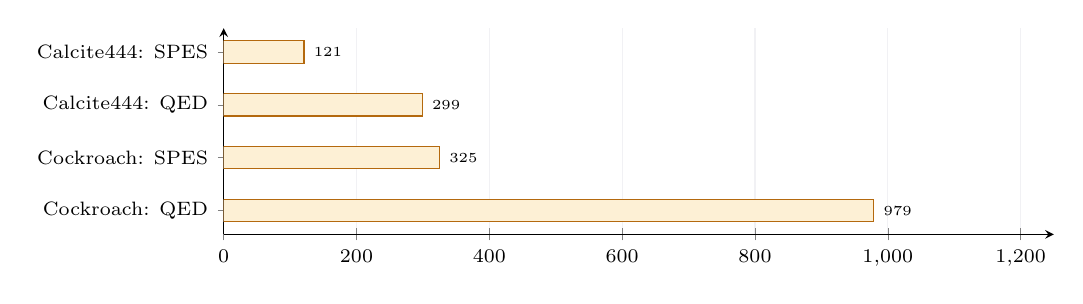
\begin{tikzpicture}
\begin{axis}[width=\textwidth,height=4.2cm,xbar,bar width=8pt,
  xmin=0,xmax=1250,
  symbolic y coords={Cockroach: QED,Cockroach: SPES,Calcite444: QED,Calcite444: SPES},
  ytick=data,tick label style={font=\scriptsize},
  nodes near coords,every node near coord/.append style={font=\tiny},
  axis lines=left,xmajorgrids,grid style={cGreyBg},enlarge y limits=0.15]
\addplot[fill=cAmberBg,draw=cAmber] coordinates
  {(979,Cockroach: QED) (325,Cockroach: SPES) (299,Calcite444: QED) (121,Calcite444: SPES)};
\end{axis}
\end{tikzpicture}\\[-2mm]
{\scriptsize Suites: Calcite v1.32 (444 pairs), CockroachDB (1287).\\
Older 232-pair Calcite suite: \udp{} 34, \spes{} 95, \QED{} 147.}
\end{column}
\begin{column}{0.46\textwidth}
\onslide<2->{{\scriptsize\textbf{where \QED{} fails} (Calcite)}\\[1mm]
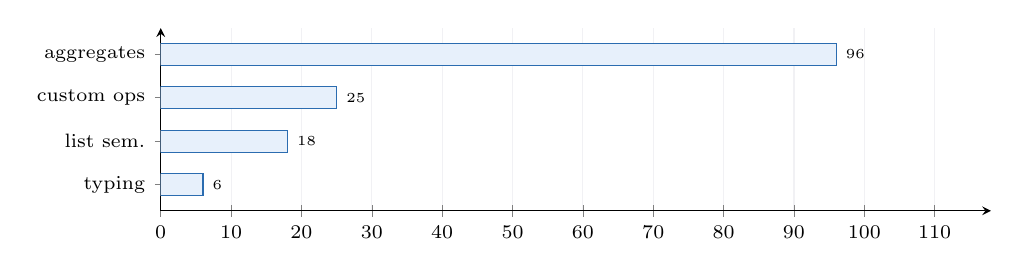
\begin{tikzpicture}
\begin{axis}[width=\textwidth,height=3.9cm,xbar,bar width=8pt,
  xmin=0,xmax=118,symbolic y coords={typing,list sem.,custom ops,aggregates},
  ytick=data,tick label style={font=\scriptsize},
  nodes near coords,every node near coord/.append style={font=\tiny},
  axis lines=left,xmajorgrids,grid style={cGreyBg},enlarge y limits=0.2]
\addplot[fill=cBlueBg,draw=cBlue] coordinates {(96,aggregates) (25,custom ops) (18,list sem.) (6,typing)};
\end{axis}
\end{tikzpicture}\\[-2mm]
{\scriptsize \alert{Aggregates dominate} --- the direct cost of leaving $\alpha$ uninterpreted.}}
\end{column}
\end{columns}
\onslide<3->{\vspace{1mm}\centering\small
Every pair \spes{} proves, \QED{} also proves. $\sim$0.88\,s average, mostly SMT time.}
\end{frame}

\sectiontitle{Part III}{U-expressions $+$ \liastar{} --- \sqlsolver{}, SIGMOD 2024}

% ------------------------------------------------------------------
\begin{frame}[fragile]{A sharper diagnosis: the unbounded summation}
Equivalence $=$ unsatisfiability of $\exists t.\,f_1(t)\neq f_2(t)$. If $f_1,f_2$ were plain
arithmetic, Z3 would settle it. \alert{They contain $\usum{}$, and no SMT solver has a theory
of unbounded sums.}
\vspace{3mm}
\onslide<2->
\begin{lstlisting}
Q1: (select x from R where y<=1000)
    union all (select x from R where y>1000 and z<500)
Q2:  select x from R where y<=1000 or z<500
\end{lstlisting}
\onslide<1->
\onslide<3->{\[f_1=\usum{t_1}E_1+\usum{t_1}E_2 \qquad\text{vs}\qquad f_2=\usum{t_1}E_3\]}
\onslide<4->{\begin{alertblock}{Two summations on the left, one on the right}
\udp{}: rejects --- term counts differ.\quad \wetune{}: no rule for $\usum{}+\usum{}$.\\[2pt]
On Calcite, 180 pairs have unbounded sums; \udp{} handles 33, \wetune{} 71.\\[2pt]
{\footnotesize (\QED{}, published later, \emph{does} get this one --- it is inside its
complete fragment. \liastar{}'s advantage is that it needs no fragment, no shared scope,
and survives aggregates and nesting.)}
\end{alertblock}}
\end{frame}

% ------------------------------------------------------------------
\begin{frame}[fragile]{\liastar{}: put the unboundedness where a solver can reach it}
\begin{block}{Additive closure}
\[S^*=\Bigl\{\vec v \;\Bigm|\; \vec v=\textstyle\sum_{i=1}^{n}\lambda_i\vec v_i,\ \vec v_i\in S,\ \lambda_i\ge0\Bigr\}\]
all non-negative combinations of members of $S$, with $n$ \alert{arbitrary}.
\end{block}
\onslide<2->{%
\begin{center}\large
$\usum{t}f(t)$ = add up $f$ over an unknown, unbounded number of tuples\\[3pt]
$S^*$ \;=\; add up an unknown, unbounded number of members of $S$
\end{center}}
\vspace{2mm}
\onslide<3->{Let $S$ be the set of possible \alert{per-tuple contribution vectors}. Then the
value of the summation is exactly an element of $S^*$.}
\vspace{2mm}
\onslide<4->{\[\liastar{}:\quad \exists\vec u,\vec v.\ F_1(\vec u,\vec v)\wedge\vec v\in\{\vec x\mid F_2(\vec x)\}^*\]
\centering NP-complete, and reducible to plain \lia{}.}
\end{frame}

% ------------------------------------------------------------------
\begin{frame}[fragile]{Five steps}
\small
\begin{enumerate}
\item<1-> Goal: $\usum{t_1}E_1+\usum{t_1}E_2\neq\usum{t_1}E_3$ unsatisfiable.
\item<2-> \alert{Vectorise}: name each sum $v_i$ and write them as \emph{one} vector sum
  \[\exists\vec v.\ v_1{+}v_2\neq v_3 \wedge (v_1,v_2,v_3)=\usum{t_1}(E_1,E_2,E_3)\]
\item<3-> Replace the vector sum by the closure:
  $\ (v_1,v_2,v_3)\in\{(x_1,x_2,x_3)\mid x_i{=}E_i\}^*$
\item<4-> Encode U-terms into \lia{}: $\ind{b}\mapsto\mathrm{ite}(b,1,0)$,
  $\sq{E}\mapsto\mathrm{ite}(E{=}0,0,1)$, every $R(t)$/attribute $\mapsto$ a fresh integer.
\item<5-> Compute \alert{generators} and emit \lia{}. Here the \texttt{ite} definitions force
  $x_1{+}x_2=x_3$, whose generators are $(1,0,1)$ and $(0,1,1)$:
  \[\vec v=\lambda_1(1,0,1)+\lambda_2(0,1,1)=(\lambda_1,\lambda_2,\lambda_1{+}\lambda_2)\]
  which forces $v_3=v_1{+}v_2$ --- contradicting $v_1{+}v_2\neq v_3$. \alert{Unsat $\Rightarrow$ equivalent.}
\end{enumerate}
\onslide<6->{\begin{alertblock}{What just happened}
No structural matching at all. \sqlsolver{} reasoned \emph{arithmetically} about three sums
sharing an index. Structural provers cannot even express that step.
\end{alertblock}}
\end{frame}

% ------------------------------------------------------------------
\begin{frame}[fragile]{Concrete aggregates --- the other half}
Every aggregate gets the same skeleton\dots
\[f(t_l\cdot t_r)=\underbrace{\ind{p(t_r)}}_{\texttt{HAVING}}\times
\underbrace{\Bigl\lVert\usum{t_1}R(t_1)\ind{t_l{=}x(t_1)}\Bigr\rVert}_{\text{group non-empty}}\times
\underbrace{(\cdots)}_{\text{the aggregate}}\]
\vspace{-3mm}
\begin{itemize}\small
\item<2-> \textsc{Sum}: $\bigl[t_r=\usum{t_1}R(t_1)\ind{t_l{=}x(t_1)}\notu{\ind{\mathit{IsNull}}}\,y(t_1)\bigr]$
      --- literally $\sum_y y\times\text{mult}$.
\item<3-> \textsc{Max}: not computed but \alert{characterised} ---
      ``nothing exceeds $t_r$'' \emph{and} ``something equals $t_r$''.
\item<4-> \textsc{Avg}: no division; assert $t_r\times\mathrm{count}=\mathrm{sum}$.
\end{itemize}
\vspace{2mm}
\onslide<5->{\begin{alertblock}{The payoff}
\texttt{select a, count(b) from R group by a} $\;\equiv\;$ \texttt{sum} of those counts
regrouped.\\
\alert{No uninterpreted-aggregate prover can ever do this} --- the needed fact is a fact
\emph{about} \textsc{Sum} and \textsc{Count}.
\end{alertblock}}
\end{frame}

% ------------------------------------------------------------------
\begin{frame}[fragile]{The catch: over-approximation}
Joins produce $\usum{}(x_1\times x_2)$ --- a product of two variables, \alert{forbidden in
\lia{}}. Fix: replace it by a fresh $y$ constrained only by $y{=}0\leftrightarrow(x_1{=}0\vee x_2{=}0)$.
\vspace{3mm}
\begin{center}
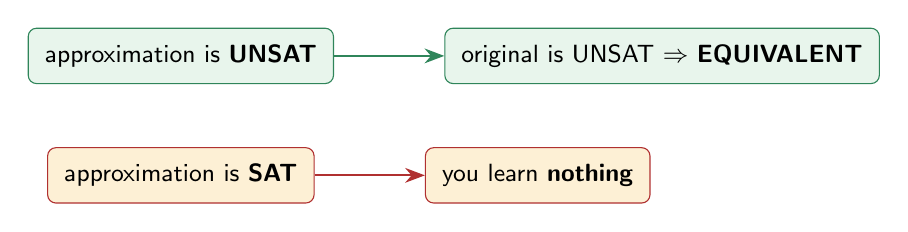
\begin{tikzpicture}[font=\small\sffamily,node distance=4mm]
\node[draw=cGreen,fill=cGreenBg,rounded corners=3pt,inner sep=6pt] (a)
  {approximation is \textbf{UNSAT}};
\node[right=14mm of a,draw=cGreen,fill=cGreenBg,rounded corners=3pt,inner sep=6pt] (b)
  {original is UNSAT $\Rightarrow$ \textbf{EQUIVALENT}};
\draw[-{Stealth[length=2.5mm]},cGreen,thick] (a)--(b);
\onslide<2->{
\node[below=8mm of a,draw=cRed,fill=cAmberBg,rounded corners=3pt,inner sep=6pt] (c)
  {approximation is \textbf{SAT}};
\node[right=14mm of c,draw=cRed,fill=cAmberBg,rounded corners=3pt,inner sep=6pt] (d)
  {you learn \textbf{nothing}};
\draw[-{Stealth[length=2.5mm]},cRed,thick] (c)--(d);}
\end{tikzpicture}
\end{center}
\vspace{3mm}
\onslide<3->{\begin{alertblock}{Implementer's warning}
A \textsc{sat} result is \alert{not} a counterexample. Report ``unknown''. If you report
``not equivalent'' your tool is unsound.
\end{alertblock}}
\onslide<4->{\centering\small Also: \lstinline|ORDER BY| is handled by a separate,
\emph{syntactic} divide-and-conquer layer --- U-expressions model bags, which have no order.}
\end{frame}

% ------------------------------------------------------------------
\begin{frame}[fragile]{\sqlsolver{} results}
\begin{columns}[T]
\begin{column}{0.48\textwidth}
{\scriptsize\textbf{Calcite} --- 232 pairs}\\[1mm]
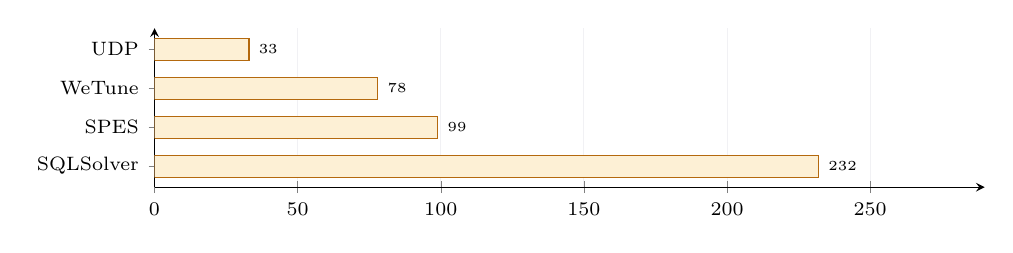
\begin{tikzpicture}
\begin{axis}[width=\textwidth,height=3.6cm,xbar,bar width=8pt,xmin=0,xmax=290,
  symbolic y coords={SQLSolver,SPES,WeTune,UDP},
  ytick=data,tick label style={font=\scriptsize},
  nodes near coords,every node near coord/.append style={font=\tiny},
  axis lines=left,xmajorgrids,grid style={cGreyBg},enlarge y limits=0.18]
\addplot[fill=cAmberBg,draw=cAmber] coordinates {(232,SQLSolver) (99,SPES) (78,WeTune) (33,UDP)};
\end{axis}
\end{tikzpicture}
\end{column}
\begin{column}{0.48\textwidth}
\onslide<2->{{\scriptsize\textbf{Spark SQL} --- 127 pairs}\\[1mm]
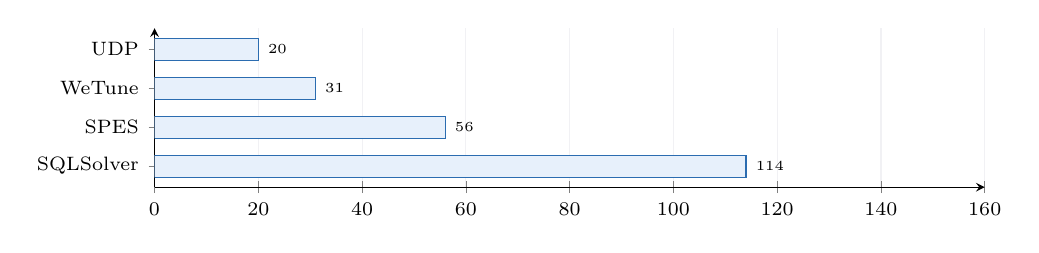
\begin{tikzpicture}
\begin{axis}[width=\textwidth,height=3.6cm,xbar,bar width=8pt,xmin=0,xmax=160,
  symbolic y coords={SQLSolver,SPES,WeTune,UDP},
  ytick=data,tick label style={font=\scriptsize},
  nodes near coords,every node near coord/.append style={font=\tiny},
  axis lines=left,xmajorgrids,grid style={cGreyBg},enlarge y limits=0.18]
\addplot[fill=cBlueBg,draw=cBlue] coordinates {(114,SQLSolver) (56,SPES) (31,WeTune) (20,UDP)};
\end{axis}
\end{tikzpicture}}
\end{column}
\end{columns}
\vspace{1mm}
\onslide<3->{\centering\small
\textbf{TPC-C} (19): \spes{} 15 $\to$ \alert{\sqlsolver{} 19}\qquad
\textbf{TPC-H} (22): \spes{} 0 $\to$ \alert{\sqlsolver{} 19}\\
{\scriptsize \udp{} and \wetune{} were not evaluated on TPC-C/TPC-H.}}
\onslide<4->{\vspace{1mm}\centering\small
Of 400 pairs the three prior provers prove 207 between them; \sqlsolver{} proves 384, a
\emph{superset}. 16 proved by nobody.}
\end{frame}

\sectiontitle{Comparison}{and what nobody has built yet}

% ------------------------------------------------------------------
\begin{frame}[fragile]{Where each system spent its effort}
\begin{center}
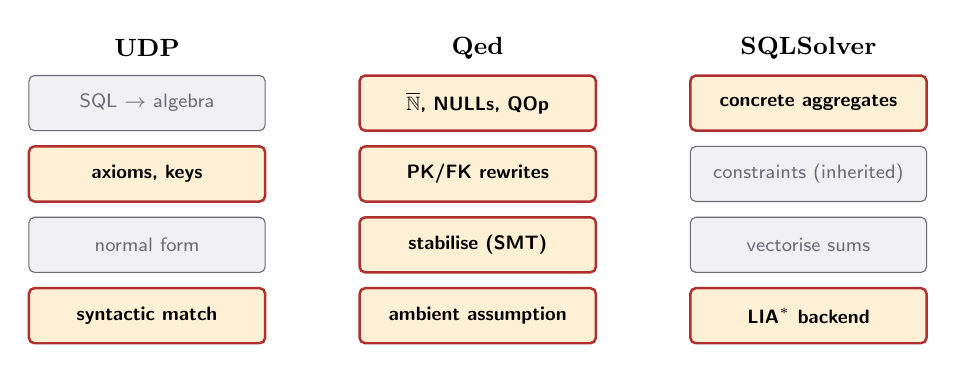
\begin{tikzpicture}[font=\scriptsize\sffamily,
  lay/.style={draw,rounded corners=2pt,minimum width=30mm,minimum height=7mm,align=center,inner sep=2pt},
  a/.style={lay,draw=cGrey,fill=cGreyBg,text=cGrey}, h/.style={lay,draw=cRed,fill=cAmberBg,line width=0.9pt}]
\node[font=\small\bfseries] at (0,2.6) {\udp{}};
\node[font=\small\bfseries] at (4.2,2.6) {\QED{}};
\node[font=\small\bfseries] at (8.4,2.6) {\sqlsolver{}};
\node[a] at (0,1.9) {SQL $\to$ algebra};
\node[h] at (0,1.0) {\textbf{axioms, keys}};
\node[a] at (0,0.1) {normal form};
\node[h] at (0,-0.8) {\textbf{syntactic match}};
\node[h] at (4.2,1.9) {\textbf{$\Nbar$, NULLs, QOp}};
\node[h] at (4.2,1.0) {\textbf{PK/FK rewrites}};
\node[h] at (4.2,0.1) {\textbf{stabilise (SMT)}};
\node[h] at (4.2,-0.8) {\textbf{ambient assumption}};
\node[h] at (8.4,1.9) {\textbf{concrete aggregates}};
\node[a] at (8.4,1.0) {constraints (inherited)};
\node[a] at (8.4,0.1) {vectorise sums};
\node[h] at (8.4,-0.8) {\textbf{\liastar{} backend}};
\end{tikzpicture}
\end{center}
\vspace{2mm}
\onslide<2->{\centering
\alert{\QED{} rebuilt the modelling and the search. \sqlsolver{} rebuilt the aggregates and
the arithmetic. They are nearly orthogonal.}}
\end{frame}

% ------------------------------------------------------------------
\begin{frame}[fragile]{A gallery of separating examples}
\small
\begin{tabular}{@{}lccc@{}}
\toprule
 & \udp{} & \QED{} & \sqlsolver{}\\
\midrule
\rowiv{1}{equal-but-different predicates}{\textcolor{cRed}{no}}{\textcolor{cGreen}{yes}}{\textcolor{cGreen}{yes}}
\rowiv{2}{aggregate pushdown through a key join\quad}{\textcolor{cRed}{no}}{\textcolor{cGreen}{yes}}{likely}
\rowiv{3}{$\usum{}+\usum{}=\usum{}$ (split union)}{\textcolor{cRed}{no}}{only in $\mathcal F_T$}{\textcolor{cGreen}{yes}}
\rowiv{4}{sum of counts $=$ one count}{\textcolor{cRed}{no}}{\textcolor{cRed}{\textbf{no}}}{\textcolor{cGreen}{yes}}
\rowiv{5}{redundant self-join on a key}{\textcolor{cRed}{no}}{\textcolor{cGreen}{yes}}{--}
\rowiv{6}{predicate pushdown, \texttt{LEFT JOIN}}{\textcolor{cRed}{no}}{\textcolor{cGreen}{yes}}{partial}
\rowiv{7}{anything with \texttt{ORDER BY}}{\textcolor{cRed}{no}}{\textcolor{cRed}{no}}{\textcolor{cGreen}{yes}}
\bottomrule
\end{tabular}
\onslide<8->{\vspace{2mm}
\begin{alertblock}{Rows 3 and 4 are the interesting ones}
Row 4 is a \emph{modelling} gap (uninterpreted aggregates); row 3 is \emph{structural}
(\QED{}'s general algorithm needs a term bijection; only its complete-fragment algorithm
relaxes that). \sqlsolver{}'s two contributions are exactly these two rows.
\end{alertblock}}
\end{frame}

% ------------------------------------------------------------------
\begin{frame}[fragile]{The root cause: squashed or not}
\begin{columns}[T]
\begin{column}{0.48\textwidth}
\textbf{\textcolor{cGreen}{Squashed}}\\
{\footnotesize \texttt{DISTINCT}, \texttt{GROUP BY}, \texttt{EXISTS}}\\[4pt]
Multiplicities are irrelevant. Push $\neq0$ inward:
\[\usum{}\rightsquigarrow\exists,\quad \times\rightsquigarrow\wedge,\quad +\rightsquigarrow\vee\]
$\Rightarrow$ a pure Boolean formula. \alert{Cheap and strong.}
\end{column}
\begin{column}{0.48\textwidth}
\onslide<2->{\textbf{\textcolor{cRed}{Not squashed}}\\
{\footnotesize plain projection, join, \texttt{UNION ALL}}\\[4pt]
Counts \emph{are} the answer, so both compare summands \alert{pointwise}:
\[(\forall\vec s.\,f{=}g)\Rightarrow \usum{\vec s}f=\usum{\vec s}g\]
\udp{} Alg.\,2 and \QED{} Alg.\,6 need a 1-to-1 term match; \QED{} Alg.\,3 only needs a
shared relational scope, but is limited to $\mathcal F_T$.}
\end{column}
\end{columns}
\vspace{3mm}
\onslide<3->{\begin{alertblock}{Why it matters}
Under a squash, $+$ becomes $\vee$ and the whole comparison is Boolean --- an SMT solver
settles it immediately. Without a squash the very same rewrite is an \alert{arithmetic}
statement about sums, and you need either alignable scopes or \liastar{}.
\end{alertblock}}
\onslide<4->{\centering\small \sqlsolver{} sidesteps the whole dichotomy: \liastar{} reasons
about the sums' \emph{values}, so no alignment is ever needed.}
\end{frame}

% ------------------------------------------------------------------
\begin{frame}[fragile]{Do not trust cross-paper numbers}
\begin{center}\large
\begin{tabular}{@{}llc@{}}
\toprule
reported by & benchmark & \spes{} scores\\\midrule
\QED{} & ``232 Calcite pairs'' & \alert{95}\\
\sqlsolver{} & ``232 Calcite pairs'' & \alert{99}\\
\bottomrule
\end{tabular}
\end{center}
\vspace{4mm}
\onslide<2->{Same baseline, same nominal benchmark, different answers --- because the
extraction pipelines differ, so the suites differ.}
\begin{itemize}\small
\item<3-> \QED{}'s harder suites (444 Calcite v1.32, 1287 CockroachDB) were never run through
      \sqlsolver{}, and vice versa.
\item<4-> \QED{} does not evaluate against \sqlsolver{} at all --- near-simultaneous work.
\item<5-> ``Proves 100\% of Calcite'' means \emph{100\% of the pairs this group extracted and
      chose to model}.
\end{itemize}
\onslide<6->{\vspace{1mm}
\begin{alertblock}{}
The only defensible comparison is one you run yourself, one extraction, all tools, same
input. \alert{Nobody has done it.}
\end{alertblock}}
\end{frame}

% ------------------------------------------------------------------
\begin{frame}[fragile]{The system nobody has built}
\begin{center}
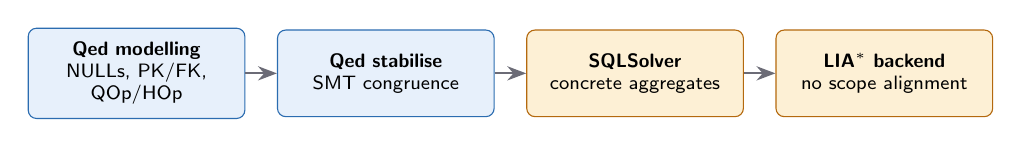
\begin{tikzpicture}[font=\scriptsize\sffamily,node distance=4mm,
  q/.style={draw=cBlue,fill=cBlueBg,rounded corners=3pt,inner sep=5pt,align=center,minimum height=11mm,text width=24mm},
  s/.style={draw=cAmber,fill=cAmberBg,rounded corners=3pt,inner sep=5pt,align=center,minimum height=11mm,text width=24mm},
  ar/.style={-{Stealth[length=2.4mm]},cGrey,thick}]
\node[q] (m) {\textbf{\QED{} modelling}\\NULLs, PK/FK,\\QOp/HOp};
\node[q,right=of m] (st) {\textbf{\QED{} stabilise}\\SMT congruence};
\node[s,right=of st] (ag) {\textbf{\sqlsolver{}}\\concrete aggregates};
\node[s,right=of ag] (li) {\textbf{\liastar{} backend}\\no scope alignment};
\draw[ar](m)--(st);\draw[ar](st)--(ag);\draw[ar](ag)--(li);
\end{tikzpicture}
\end{center}
\vspace{4mm}
\begin{itemize}
\item<2-> \QED{}'s term-bijection step is its ceiling. \alert{\liastar{} removes exactly that
      ceiling.}
\item<3-> \QED{}'s uninterpreted $\hop$ is its largest failure bucket (96 Calcite cases).
      \alert{\sqlsolver{}'s aggregate tables fill it.}
\item<4-> \sqlsolver{}'s weakest areas --- NULLs, constraints, unknown operators --- are
      \alert{precisely \QED{}'s contributions.}
\end{itemize}
\end{frame}

% ------------------------------------------------------------------
\begin{frame}[fragile]{If you are implementing this}
\textbf{Build order} (do not start with the fancy parts):
\begin{enumerate}\small
\item<2-> plan $\to$ algebra for \texttt{Scan/Filter/Project/Join/Union} only
\item<3-> normalisation to sum-of-products (pure syntax, no solver)
\item<4-> pointwise term matching with scope permutation
\item<5-> \alert{bring in SMT for predicates} --- biggest capability jump per line of code
\item<6-> \alert{stabilisation via congruence classes} --- second biggest
\item<7-> primary keys (one rewrite, large payoff), then squash / \texttt{GroupBy}
\item<8-> only then: NULLs, foreign keys, unknown operators, \liastar{}
\end{enumerate}
\onslide<9->{\vspace{2mm}
\begin{alertblock}{Test against a real database}
Generate tiny instances with \alert{heavy duplicates and NULLs}; compare with
\texttt{EXCEPT ALL} both ways; and \alert{evaluate your algebra directly} on the same
instance to validate the \emph{translation}, not just the decision procedure.\\[2pt]
Our running example must produce $(1,60)$ vs two copies of $(1,30)$. If yours doesn't, the
\texttt{GroupBy} or key rule is wrong.
\end{alertblock}}
\end{frame}

% ------------------------------------------------------------------
\begin{frame}[standout]
Three ideas worth remembering
\end{frame}

\begin{frame}[fragile]{Takeaways}
\begin{enumerate}
\item<1-> \textbf{A table is a counting function.} Filtering is multiplication, union is
      addition, projection is an unbounded sum. Every system here is a different way of
      comparing two such formulas.
\vspace{2mm}
\item<2-> \textbf{The two 2024 systems solve different halves.}\\
      \QED{} $=$ better \emph{model} of SQL (NULLs, keys, unknown operators, context-sensitive
      subquery checks).\\
      \sqlsolver{} $=$ better \emph{arithmetic} (unbounded sums via \liastar{}, real
      aggregates).
\vspace{2mm}
\item<3-> \textbf{Squash is the dividing line.} Under a squash, equivalence is a Boolean
      question an SMT solver answers instantly. Without one, it is an arithmetic question
      about sums --- and that is where the frontier is.
\end{enumerate}
\vspace{4mm}
\onslide<4->{\centering\small
Primary key $\to$ $\sq{S(a)}$ $\to$ \texttt{Inner Unique: true}. The optimiser and the prover
are tracking the same fact for different reasons.}
\end{frame}

\end{document}
